\documentclass[tikz,border=5pt]{standalone}
\usepackage{pgfplots}
\pgfplotsset{compat=1.18}
\definecolor{corba}{HTML}{365FB3}\definecolor{guia}{HTML}{7C3AED}\definecolor{punt}{HTML}{B91C1C}
\begin{document}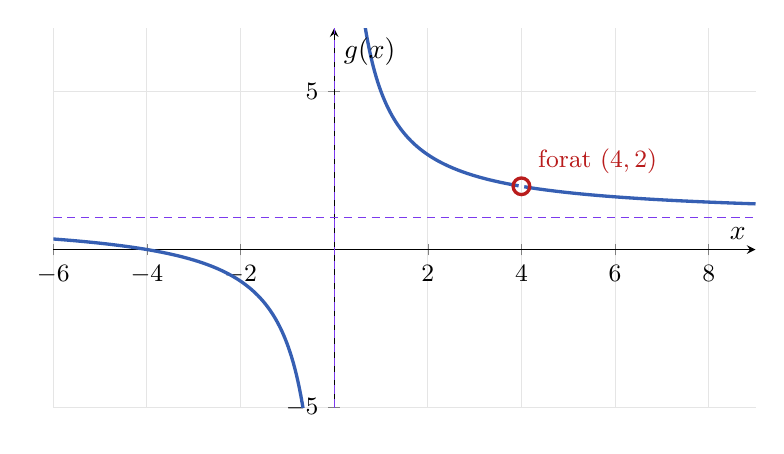
\begin{tikzpicture}
\begin{axis}[width=10.5cm,height=6.4cm,axis lines=middle,xmin=-6,xmax=9,ymin=-5,ymax=7,
 xlabel={$x$},ylabel={$g(x)$},grid=major,grid style={black!10},tick label style={font=\small},clip=true]
 \addplot[corba,very thick,domain=-6:-0.08,samples=180]{(x+4)/x};
 \addplot[corba,very thick,domain=0.08:3.94,samples=180]{(x+4)/x};
 \addplot[corba,very thick,domain=4.06:9,samples=180]{(x+4)/x};
 \addplot[guia,densely dashed] coordinates {(0,-5) (0,7)};
 \addplot[guia,densely dashed,domain=-6:9]{1};
 \addplot[only marks,mark=o,mark size=3pt,very thick,punt,fill=white] coordinates {(4,2)};
 \node[anchor=south west,font=\small,text=punt] at (axis cs:4.15,2.1) {forat $(4,2)$};
\end{axis}\end{tikzpicture}\end{document}
